\documentclass[10pt]{article}
\usepackage[margin=0.78in]{geometry}
\usepackage[T1]{fontenc}
\usepackage{lmodern}
\usepackage{microtype}
\usepackage{graphicx}
\usepackage{booktabs}
\usepackage{placeins}
\usepackage{xcolor}
\usepackage{hyperref}
\definecolor{navy}{HTML}{16324F}
\definecolor{teal}{HTML}{087E8B}
\hypersetup{colorlinks=true,linkcolor=navy,urlcolor=teal}
\title{\textcolor{navy}{When Should IDM-Viz Refit?}\\[3pt]\large A Label-Safe Schedule Audit}
\author{23I-2581 and 23I-2604\\Data Analysis and Visualization --- Phase 3 addendum}
\date{17 November 2026}
\begin{document}\maketitle
\begin{abstract}
This controlled extension compares a frozen logistic classifier with periodic and released-error-triggered global refitting. It tests whether the trigger avoids unnecessary stationary-stream updates and whether either schedule recovers useful accuracy after a synthetic conditional reversal. Thirty paired seeds, three label delays, and two synthetic mechanisms are used. The study evaluates global refitting only; it is not an evaluation of region-local adaptation or a claim of operational benefit.
\end{abstract}
\section{Protocol}
The stream contains 96 batches of 500 observations. A single logistic classifier is trained on the frozen historical set; its scaler is fit on historical training rows. The periodic policy refits at forecast clocks 25, 49, and 73. The triggered policy requires both latest released source cohorts to exceed the historical calibration error by 0.10, has an eight-clock cooldown, and is capped at three updates. Each update uses historical training rows plus at most the latest 2,000 released monitoring labels. The trigger threshold is fixed from calibration data; it is not selected on monitoring outcomes.

For delay $d$, source batch $s$ is available before forecast batch $b$ only when $s+d<b$. The current batch is predicted before its labels can be released. The detector uses stored predictions only after the scheduled release. The primary unit for uncertainty is the seed: batch metrics are aggregated within each seed, then a paired seed bootstrap forms 95\% intervals.

\section{Results}
\begin{figure}[ht]
\centering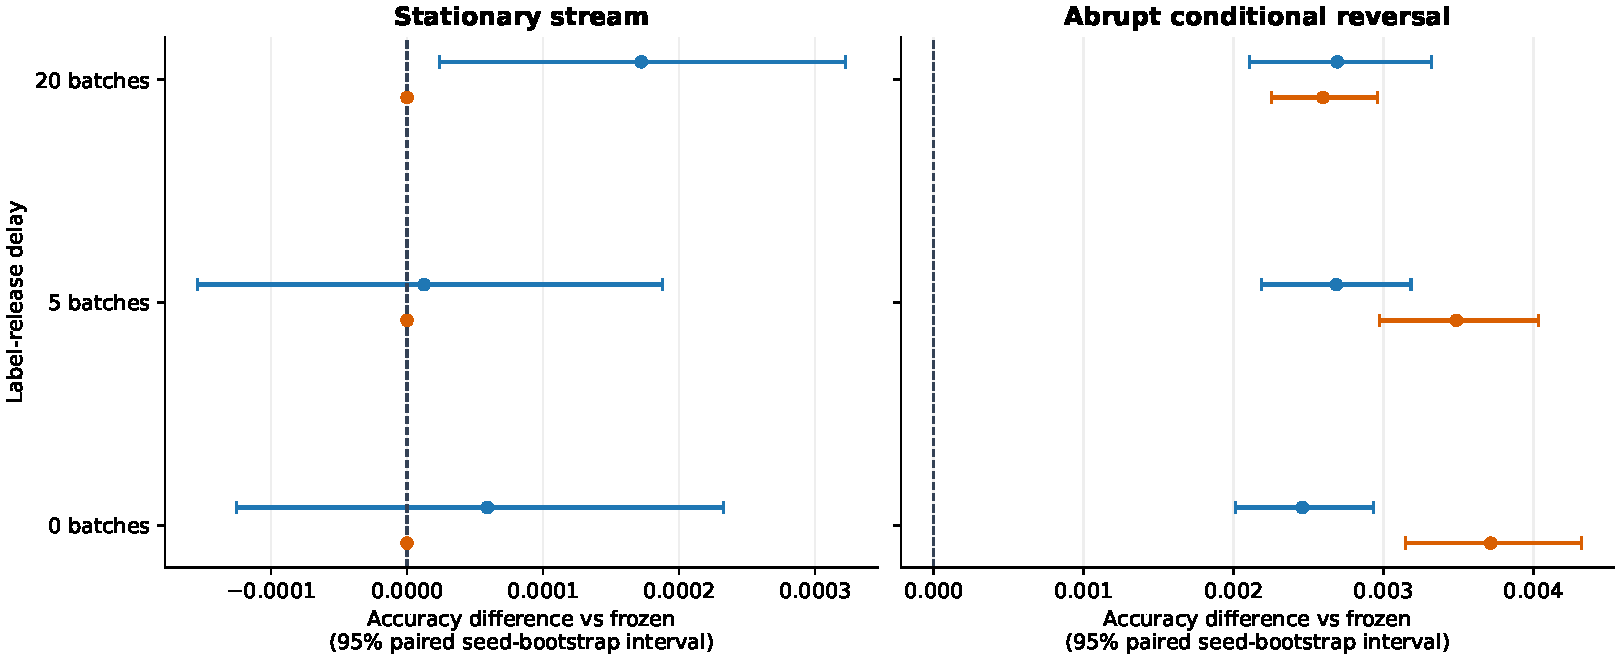
\includegraphics[width=\linewidth]{adaptation_schedule.pdf}
\caption{Paired accuracy differences from the frozen policy; blue denotes periodic refitting and orange the released-error trigger. Intervals resample the 30 matched seeds.}
\end{figure}
\begin{table}[ht]
\centering\small
\begin{tabular}{@{}llrrrr@{}}
\toprule
Mechanism & Delay & Frozen & Periodic & Triggered & Trigger updates\\
\midrule
Stationary & 0 & 0.724 & 0.725 & 0.724 & 0.0\\
Stationary & 5 & 0.724 & 0.724 & 0.724 & 0.0\\
Stationary & 20 & 0.724 & 0.725 & 0.724 & 0.0\\
Reversal & 0 & 0.388 & 0.390 & 0.391 & 3.0\\
Reversal & 5 & 0.388 & 0.390 & 0.391 & 3.0\\
Reversal & 20 & 0.388 & 0.390 & 0.390 & 3.0\\
\bottomrule
\end{tabular}
\caption{Mean accuracy across paired seeds; trigger updates are averaged across seeds.}
\end{table}

The trigger did not update in the stationary condition, while periodic refitting used all three update slots. Under abrupt reversal, the trigger fired three times at each tested delay. Both adaptation schedules produced only modest gains in all-stream accuracy over the frozen classifier. Gains were smaller under longer label delay, consistent with less timely evidence. These are controlled synthetic results, not proof of generally effective adaptation. Read the adjacent \texttt{paired\_accuracy\_differences.csv} for seed-paired estimates and intervals.

\FloatBarrier
\section{Interpretation and limits}
This extension adds a global error-triggered schedule to the existing periodic comparison. It does not assess region-local refitting, multiple real-world streams, multiple classifiers, concept-change recovery guarantees, or equal consumed-label budgets against a frozen policy (which consumes no monitoring labels for fitting). The cumulative update rule and trigger are deliberately simple. The outcome is therefore a bounded policy comparison, not a leaderboard. Fit-row counts are a computational proxy, not wall-clock or energy measurements. Synthetic reversal results cannot establish utility for a real deployment.

\section{Reproduction}
Run from the workspace root:
\begin{verbatim}
powershell -NoProfile -ExecutionPolicy Bypass \\
  -File .\\scripts\\reproduce_adaptation_schedule_audit.ps1
\end{verbatim}
The runner receipt records code/configuration and output hashes, label-release semantics, seed bank and software versions. Contract tests check that no forecast consumes same-clock labels and that the result tables contain all locked seed-policy cells.

\end{document}
